\subsection{UC1 - Creazione ambiente}
\label{sub:uc2}

%TODO: Add correct image
\begin{figure}[h]
    \centering
    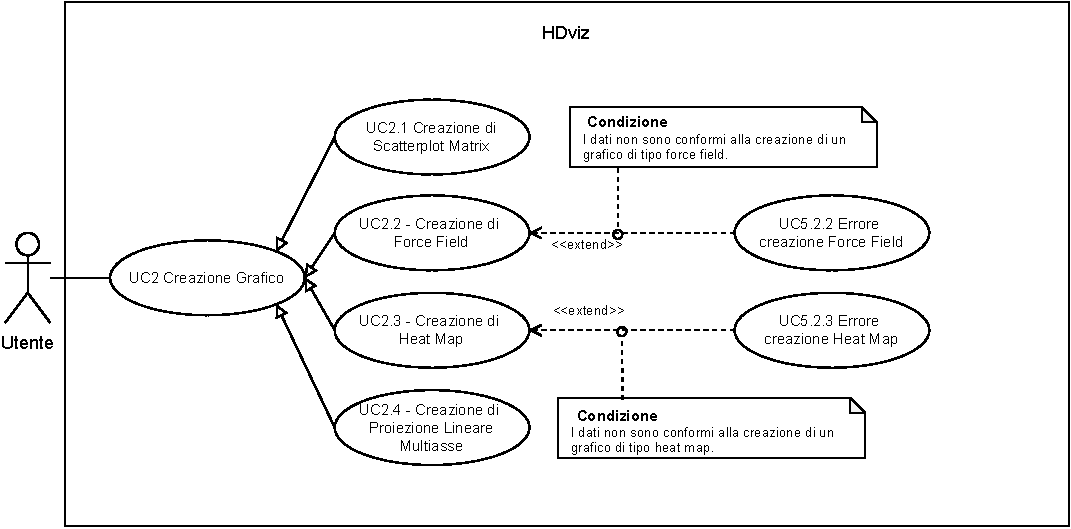
\includegraphics[width=0.5\textwidth]{componenti/casi-duso/diagrammi/UC2.pdf}
    \caption{Diagramma rappresentante UC3}
    \label{fig:UC2}
\end{figure}


\begin{itemize}
    \item \textbf{Descrizione}: L'utente prepara l'applicativo HDviz alla rappresentazione
                                grafica dei dati importando l'opportuno dataset e assegna, 
                                se non già definiti, dei metadati 
                                che descrivono il tipo del dato di ogni colonna.
	
    \item \textbf{Attore primario}: Utente;
    
    \item \textbf{Precondizione}:   L'utente decide di caricare i dati.

    \item \textbf{Postcondizione}:  Viene caricato un dataset. 
    
                                    Ogni colonna del dataset ha associato
                                    un metatag che indica la tipologia del dato;

	\item \textbf{Scenario principale}:
		\begin{enumerate}
			\item L'utente seleziona l'opzione di aggiunta dei dati;
            \item L'utente seleziona la fonte dei dati da importare: (UC1.1)
            \begin{itemize}
                \item L'utente ha scelto di reperire i dati mediante file (UC1.1.1)
                \item L'utente ha scelto di reperire i dati da database (UC1.1.2)
            \end{itemize}
        \end{enumerate}
    %TODO: Rimuovo da qui e metto ad ogni use case che è coinvolto il suo? Non sarebbe corretto
    % magari in quanto la post non sarebbe poi più rispettata.
    \item \textbf{Estensioni}:
        \begin{enumerate}
            \item L'utente importa un file di un formato non valido oppure vuoto:
            \begin{enumerate}
                \item La creazione del dataset fallisce.
                \item Viene visualizzato il messaggio di errore. (UC1.1.1e)
            \end{enumerate}
            \item L'operazione sul database fallisce:
            \begin{enumerate}
                \item La creazione del dataset fallisce.
                \item Viene visualizzato il messaggio di errore. (UC1.1.2e)
            \end{enumerate}
            \item Il dataset caricato presenta metatag non validi o ne è provvisto:
            \begin{enumerate}
                \item L'utente inserisce manualmente un metatag per ogni colonna del dataset. (UC1.2)
            \end{enumerate}
        \end{enumerate}
\end{itemize}


\subsection{UC1.1 - Inserimento dati}
\begin{itemize}
    \item \textbf{Descrizione}: L'utente importa un dataset provvisto
                                di metatag validi per il corretto utilizzo del programma.

    \item \textbf{Attore primario}: Utente;
    
    \item \textbf{Precondizione}:   L'utente decide di caricare i dati.

    \item \textbf{Postcondizione}:  Viene caricato un dataset. 

                                    Ogni colonna del dataset ha associato
                                    un metatag che indica la tipologia del dato;

	\item \textbf{Scenario principale}:
		\begin{enumerate}
			\item L'utente seleziona l'opzione di aggiunta dei dati;
            \begin{itemize}
                \item L'utente sceglie di importare i dati da file (UC1.1.1);
                \item L'utente seleziona di importare i dati da database (UC1.1.2);
            \end{itemize}
            
        \end{enumerate}
    %TODO: Aggiungere scenario secondario qui?
    \item \textbf{Estensioni}:
        \begin{enumerate}
            \item Il dataset caricato presenta metatag non validi o ne è provvisto:
            \begin{enumerate}
                \item L'utente inserisce manualmente un metatag per ogni colonna del dataset. (UC1.2)
            \end{enumerate}    
        \end{enumerate}
\end{itemize}

\subsection{UC1.1.1 - Inserimento dati da file}
\begin{itemize}
    \item \textbf{Descrizione}: L'utente importa un dataset non vuoto da un file del suo dispostivo.

    \item \textbf{Attore primario}: Utente;
    
    \item \textbf{Precondizione}:   L'utente selezione l'opzione di caricare i dati.

    \item \textbf{Postcondizione}:  Viene caricato un dataset da file. 

                                    Ogni colonna del dataset ha associato
                                    un metatag che indica la tipologia del dato;

	\item \textbf{Scenario principale}:
		\begin{enumerate}
			\item L'utente seleziona l'opzione di aggiunta dei dati mediante file;
			\item L'utente seleziona file di dati da importare;
        \end{enumerate}

    \item \textbf{Estensioni}
    \begin{enumerate}
  
    \item L'utente importa un file di un formato non valido oppure vuoto:
        \begin{enumerate}
            \item La creazione del dataset fallisce.
            \item Viene visualizzato il messaggio di errore. (UC1.1.1e)
        \end{enumerate}
    \end{enumerate}
\end{itemize}

\subsection{UC1.1.2 - Inserimento dati da database}
\begin{itemize}
    \item \textbf{Descrizione}: L'utente importa un dataset non vuoto dal database.

    \item \textbf{Attore primario}: Utente;
    
    \item \textbf{Attore secondario}: Database; 
    
    \item \textbf{Precondizione}:   L'utente decide di caricare i dati.

    \item \textbf{Postcondizione}:  Viene caricato un dataset dal database. 

                                    Ogni colonna del dataset ha associato
                                    un metatag che indica la tipologia del dato;

	\item \textbf{Scenario principale}:
		\begin{enumerate}
			\item L'utente seleziona l'opzione di aggiunta dei dati mediante accesso al database;
			\item L'utente seleziona i dati da importare;
        \end{enumerate}

    \item \textbf{Estensioni}:
        \begin{enumerate}
            \item L'operazione sul database fallisce:
            \begin{enumerate}
                \item La creazione del dataset fallisce.
                \item Viene visualizzato il messaggio di errore. (UC1.1.2e)
            \end{enumerate}  
         \end{enumerate}
\end{itemize}



\subsection{UC1.2 - Inserimento metadati}
\begin{itemize}
    \item \textbf{Descrizione}: L'utente assegna ad ogni colonna del dataset importato,
                                in cui non è già correttamente definito,
                                un metadato che ne descrive la tipologia del dato;


    \item \textbf{Attore primario}: Utente;
    
    \item \textbf{Precondizione}:   L'utente ha caricato un dataset e non tutti i suoi 
                                    metatag sono validi o definiti.

    \item \textbf{Postcondizione}:  Il dataset caricato è provvisto di metatag validi. 

	\item \textbf{Scenario principale}:
		\begin{enumerate}
			\item L'utente assegna ad ogni colonna del dataset il tipo di dato che rappresenta (metatag);
        \end{enumerate}

\end{itemize}

